\documentclass[8pt]{beamer}
\usepackage[utf8]{inputenc}
\usepackage{ulem}
\usepackage{xcolor}
\usepackage{colortbl}
\usepackage{epsfig}
% \usepackage{cancel}
\usepackage{ulem}
% \usepackage{threeparttable} % Joao Pela: 
\usepackage{amsmath}
\usepackage{hyperref}
\usepackage{appendixnumberbeamer}
\usepackage{pdfpages}
% \usepackage{feynmp}         % For latex produced Feynman Diagrams

% Rule for feynmp diagrams to be considered graphics
% \DeclareGraphicsRule{*}{mps}{*}{}
% 
% % New compile sequence for feynmp
% \makeatletter
% \def\endfmffile{%
%   \fmfcmd{\p@rcent\space the end.^^J%
%           end.^^J%
%           endinput;}%
%   \if@fmfio
%     \immediate\closeout\@outfmf
%   \fi
%   \ifnum\pdfshellescape=\@ne
%     \immediate\write18{mpost \thefmffile}%
%   \fi}
% \makeatother

\usetheme{Madrid}

\author[J. Pela]{J. Pela}
\title{L1 Rates Estimation for 2015 (Legacy System)}
\institute[ICL]{Imperial College London}
\date{2014-07-01}

% The log drawn in the upper right corner.
\logo{\includegraphics[height=0.115\paperheight]{img/Logo_CMSICL.png}}

\begin{document}
\setlength{\unitlength}{1mm}

% ###################################################
\begin{frame}
  \titlepage
\end{frame}

% ###################################################
\begin{frame}{Today's presentation}
 
\begin{block}{Topics}
 
\begin{itemize}
  \item L1 Rates Estimation for 2015 with the legacy system
  \item Problems and issues found.
\end{itemize}

\end{block}

\end{frame}

% ###################################################
\begin{frame}{Neutrino Gun}

\begin{block}{Base idea}
 
For studying of L1T Rates the normal procedure is using neutrino gun samples. :
\begin{itemize}
 \item Hard process is invisible (only a neutrino is fired through the experiment)
 \item Event consists only of PU (overlapped Minimum/Zero bias events)
 \item Recreated the vast majority of events at the fire the L1T
 \item Caveat: Does not contain any real hard scattering events therefore HLT studies cannot be done with them.
\end{itemize}

\end{block}

\begin{block}{Method}
 
\begin{itemize}
 \item Determine algorithm event selection efficiency, this will be the probability of a bunch firing.
 \item Each bunch firing will represent 11246 Hz, so we apply efficiency and obtain rate per bunch.
 \item We multiply per number of bunches on the machine to obtain algorithm pure rate (no overlapping with other algorithm)
\end{itemize}
 
\end{block}

\end{frame}
                                                                                                                              
% ###################################################
\begin{frame}{Neutrino Gun - Efficiency per bunch}

\begin{block}{L1T}
\centering

\begin{tabular}{|l|c|c|c|}
\hline
L1T Algo   & PU20bx25 & PU40bx50 & PU40bx25 \\
\hline \hline
L1\_ETM30  & 0.010484 & 0.048612 & 0.099137 \\                                                                                                                                                                                                                                                        
L1\_ETM36  & 0.003417 & 0.018527 & 0.044528 \\                                                                                                                                                                                                                                                       
L1\_ETM50  & 0.000418 & 0.002087 & 0.006257 \\                                                                                                                                                                                                                                                      
L1\_ETM70  & 0.000058 & 0.000193 & 0.000427 \\
L1\_ETM100 & 0.000009 & 0.000023 & 0.000027 \\                                                                                                                                                                                                                   
\hline
\end{tabular}

\end{block}

\begin{block}{HLT (Just for indicative purposes)}
 
\resizebox{\linewidth}{!}{ 
\begin{tabular}{|l|c|c|c|}
\hline
HLT Algo                                                & PU20bx25 & PU40bx50 & PU40bx25  \\
\hline\hline                                                                                                                                                                                                                                                                      
HLT\_DiPFJet40\_PFMETnoMu65\_MJJ800VBF\_AllJets\_v      & 0.000003 & 0.000008 & 0.000034  \\                                                                                                                                                                                                                 
HLT\_DiPFJet40\_PFMETnoMu65\_MJJ600VBF\_LeadingJets\_v  & 0.000004 & 0.000012 & 0.000060  \\
\hline\hline                                                                                                                                                                      
HLT\_DiJet20\_MJJ650\_AllJets\_DEta3p5\_HT120\_VBF\_v   & 0.000141 & 0.000422 & 0.000247  \\                                                                                                                                                                                                              
HLT\_DiJet30\_MJJ700\_AllJets\_DEta3p5\_VBF\_v          & 0.000093 & 0.000238 & 0.000118  \\                                                                                                                                                                                                                    
HLT\_DiJet35\_MJJ650\_AllJets\_DEta3p5\_VBF\_v          & 0.000095 & 0.000224 & 0.000131  \\                                                                                                                                                                                                                    
HLT\_DiJet35\_MJJ700\_AllJets\_DEta3p5\_VBF\_v          & 0.000076 & 0.000176 & 0.000093  \\                                                                                                                                                                                                                    
HLT\_DiJet35\_MJJ750\_AllJets\_DEta3p5\_VBF\_v          & 0.000064 & 0.000148 & 0.000072  \\  
\hline
\end{tabular}
}

\end{block}

We can already notice at L1 that there is a significant increase in efficiency from 50 ns to 25 ns with PU 40. More in next slides... 

\end{frame}

% ###################################################
\begin{frame}{Neutrino Gun - Rate per bunch}

\begin{block}{L1T}
\centering

\begin{tabular}{|l|c|c|c|}
\hline
L1T Algo   & PU20bx25 & PU40bx50 & PU40bx25 \\
\hline \hline
L1\_ETM30  & 117.9057 & 546.6908 & 1114.890 \\                                                                                                                                                                                                                                                        
L1\_ETM36  & 38.4230  & 208.3502 & 500.7619 \\                                                                                                                                                                                                                                                       
L1\_ETM50  & 4.706185 & 23.47229 & 70.36284 \\                                                                                                                                                                                                                                                      
L1\_ETM70  & 0.649494 & 2.175597 & 4.799815 \\
L1\_ETM100 & 0.102957 & 0.263129 & 0.304293 \\                                                                                                                                                                                                                   
\hline
\end{tabular}

\end{block}

\begin{block}{HLT (Just for indicative purposes)}
 
\resizebox{\linewidth}{!}{ 
\begin{tabular}{|l|c|c|c|}
\hline
HLT Algo                                                &  PU20bx25 & PU40bx50 & PU40bx25  \\
\hline\hline                                                                                                                                                                                                                                                                       
HLT\_DiPFJet40\_PFMETnoMu65\_MJJ800VBF\_AllJets\_v      &  0.028866 & 0.092095 & 0.382027  \\                                                                                                                                                                                                                 
HLT\_DiPFJet40\_PFMETnoMu65\_MJJ600VBF\_LeadingJets\_v  &  0.041375 & 0.130368 & 0.671807  \\
\hline\hline                                                                                                                                                                       
HLT\_DiJet20\_MJJ650\_AllJets\_DEta3p5\_HT120\_VBF\_v   &  1.580916 & 4.744692 & 2.777506  \\                                                                                                                                                                                                              
HLT\_DiJet30\_MJJ700\_AllJets\_DEta3p5\_VBF\_v          &  1.046888 & 2.673150 & 1.324180  \\                                                                                                                                                                                                                    
HLT\_DiJet35\_MJJ650\_AllJets\_DEta3p5\_VBF\_v          &  1.069019 & 2.514077 & 1.476450  \\                                                                                                                                                                                                                    
HLT\_DiJet35\_MJJ700\_AllJets\_DEta3p5\_VBF\_v          &  0.858294 & 1.978251 & 1.048176  \\                                                                                                                                                                                                                    
HLT\_DiJet35\_MJJ750\_AllJets\_DEta3p5\_VBF\_v          &  0.718773 & 1.661300 & 0.808579  \\  
\hline
\end{tabular}
}

\end{block}

Here we can see that difference int the rate per bunch which at ETM30 doubles the rate and at ETM100 give an 15\% increase.

\end{frame}

% ###################################################
\begin{frame}{Neutrino Gun - Maximum Pure Rate}

We can now apply the maximum number of bunch for each configuration which is 2808 for 25 ns and 1380 for 50 ns and calculate maximum pure 

\begin{block}{L1T}
\centering

\begin{tabular}{|l|c|c|c|}
\hline
L1T Algo   &   PU20bx25 &   PU40bx50 &   PU40bx25 \\
\hline \hline
L1\_ETM30  &  331079.35 &  754433.44 & 3130611.86 \\                                                                                                                                                                                                                                                        
L1\_ETM36  &  107892.05 &  287523.31 & 1406139.58 \\                                                                                                                                                                                                                                                       
L1\_ETM50  &   13214.97 &   32391.76 &  197578.86 \\                                                                                                                                                                                                                                                      
L1\_ETM70  &    1823.78 &    3002.32 &   13477.88 \\
L1\_ETM100 &     289.10 &     363.12 &     854.46 \\                                                                                                                                                                                                                   
\hline
\end{tabular}

\end{block}

\begin{block}{HLT (Just for indicative purposes)}
 
\resizebox{\linewidth}{!}{ 
\begin{tabular}{|l|c|c|c|}
\hline
HLT Algo                                                & PU20bx25 & PU40bx50 & PU40bx25  \\
\hline\hline                                                                                                                                                                                                                                                                      
HLT\_DiPFJet40\_PFMETnoMu65\_MJJ800VBF\_AllJets\_v      &    81.06 &   127.09 &  1072.73  \\                                                                                                                                                                                                                 
HLT\_DiPFJet40\_PFMETnoMu65\_MJJ600VBF\_LeadingJets\_v  &   116.18 &   179.91 &  1886.43  \\
\hline\hline                                                                                                                                                                      
HLT\_DiJet20\_MJJ650\_AllJets\_DEta3p5\_HT120\_VBF\_v   &  4439.21 &  6547.67 &  7799.24  \\                                                                                                                                                                                                              
HLT\_DiJet30\_MJJ700\_AllJets\_DEta3p5\_VBF\_v          &  2939.66 &  3688.95 &  3718.30  \\                                                                                                                                                                                                                    
HLT\_DiJet35\_MJJ650\_AllJets\_DEta3p5\_VBF\_v          &  3001.80 &  3469.43 &  4145.87  \\                                                                                                                                                                                                                    
HLT\_DiJet35\_MJJ700\_AllJets\_DEta3p5\_VBF\_v          &  2410.09 &  2729.99 &  2943.28  \\                                                                                                                                                                                                                    
HLT\_DiJet35\_MJJ750\_AllJets\_DEta3p5\_VBF\_v          &  2018.32 &  2292.59 &  2270.49  \\  
\hline
\end{tabular}
}

\end{block}

Since rates at 25 ns are already higher with a higher number of bunches the rate explodes. Notice that our triggers at HLT level at 25 ns just with neutrino guns all pass 1 kHz.

\end{frame}

% ###################################################
\begin{frame}{Understanding higher rates from 25 to 50 ns}
 
I have identified several possible reason for this higher rates
\begin{block}{HLT}
 
\begin{itemize}
  \item Higher out of time pile up (OOT PU) due to higher bunch density and bunch to bunch interaction which will add events to calorimeters
  \item Saturation of ECAL or HCAL primitives and/or RCT zones
  \item High integration times by HCAL or ECAL systems (more OOT PU recorded or even more bx) 
\end{itemize}

\end{block}
 
Most like likely a combination of all of this effects.
 
\begin{block}{Steps taken}
 
\begin{itemize}
  \item Contacted HCAL and Trigger Calorimeter experts and indeed we integrate for 50ns the energy so energy on the next event at 25 ns will be in pratice OOT PU always...
  \item Recent studies have showed (see 2 weeks ago L1 DPG meeting) HCAL, ECAL or RCT saturation is now an issue and will generate ETM.
  \item I am in contact with people upgrading algorithms so we can profit from this.
\end{itemize}

\end{block} 
 
\end{frame}

% ###################################################
\begin{frame}{Summary and next steps}
 
\begin{block}{Summary:}
 
\begin{itemize}
  \item A study for rates with the legacy system is underway and already can see 25 ns will present some difficulties. Similar effects already observed in the signal efficiency study.
  \item Several issue contribute to make rates explode specially for 25 ns.
\end{itemize}

\end{block}

\begin{block}{Next Steps:}
 
\begin{itemize}
  \item Finish L1 legacy study and do HLT full study
  \item Do UCT study
  \item Include new features for future HLT Paths (PU subtracting, etc) 
\end{itemize}
 
\end{block}

\end{frame}

% ###################################################
\appendix
% ###################################################
\begin{frame}
 
\begin{block}

\begin{center}Backup Slides\end{center}

\end{block}

\end{frame}

% {
% \setbeamercolor{background canvas}{bg=}
% \includepdf[pages=11]{hinv_magnan_140506.pdf}
% }

\end{document}